\chapter{Experimentación}\label{chapter:experiments}

En este capítulo se presentan tres marcos experimentales con el objetivo de verificar que es posible evaluar sistemas Auto-ML en los conjuntos de datos de 
\textit{HAutoML-Bench}. 

El primer marco (\ref{section:data}) muestra un análisis visual de las propiedades que presentan dichos conjuntos con el propósito de demostrar que existe complejidad y 
diversidad en sus propiedades. Esto asegura que se tiene un conjunto de calidad en donde su estrategia de creación mitiga los sesgos de 
selección.

Los dos marcos restantes proponen una evaluación cualitativa y cuantitativa de los sistemas de aprendizaje de máquinas automatizados.
La evaluación cualitativa (\ref{section:qualitative}) tiene el fin de analizar las características de algunas herramientas Auto-ML para determinar cuáles 
poseen las funcionalidades necesarias para evaluarse en cada uno de los conjuntos de \textit{HAutoML-Bench}.

El último marco (\ref{section:quantitative}), efectúa las mediciones de rendimiento de los sistemas seleccionados en el marco experimental anterior. En su inicio 
se especifican las diferentes etapas de evaluación y sus configuraciones (\ref{subsection:seetings}). Luego se presentan los valores de 
rendimiento obtenidos y las comparaciones realizadas (\ref{subsection:results}).

En la última sección se discuten los resultados de cada uno de los marcos experimentales (\ref{subsection:discussions}).  

\section{Análisis de los Conjuntos de Datos}\label{section:data}

\textit{HAutoML-Bench} recoge 11 conjuntos multimodales y 16 conjuntos de texto puro.
La estrategia de selección de estos conjuntos asegura ser un reto para los sistemas Auto-ML ya que existe una mezcla de dominios y una gran presencia de datos no 
estructurados.

En las figuras \ref{fig:columns-t},\ref{fig:columns-d},\ref{fig:columns-i} y \ref{fig:columns-e} se muestra la frecuencia de datos no estructurados presentes en 
los conjuntos. 
Estas propiedades adquieren más complejidad al unirse con las característica tabulares\footnote{Columnas que son numéricas,booleanas y categóricas} 
(\ref{fig:columns-n},\ref{fig:columns-b},\ref{fig:columns-c}).

\textit{HAutoML-Bench} presenta variedad es sus metacaracterísticas e incluye ciertas propiedades que provocan 
un bajo rendimiento en los sistemas, ejemplo el desbalance.

La figura \ref{fig:columns} muestra los diferentes números de columnas que presentan los conjuntos, siendo \textit{google-guest} el mayor con 40 columnas. 
Predominan los conjuntos con 2 y 3 columnas. 
Con respecto a la cantidad de instancias (\ref{fig:instances}) se puede ver que hay conjuntos de diferentes tamaños.
El mayor de todos es \textit{project-kickstarter} y el menor es \textit{wnli-es}.
Los valores faltantes (\ref{fig:null}) están presentes en la minoría de los conjuntos; sin embargo, en cada uno de ellos hay una 
gran cantidad de los mismos. 
En los ejemplos de clasificación existe un balance entre el número de conjuntos de clasificación binaria y de multiclase (\ref{fig:clases}). 
También, existe un gran número de conjuntos que tienen un desequilibrio de clases con un índice menor que 0.4 (\ref{fig:balance}).


\begin{figure}
  \begin{minipage}[b]{0.31\textwidth}
    \centering
    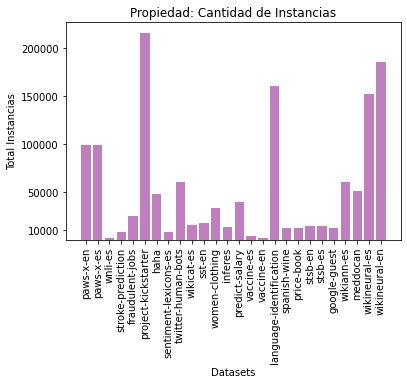
\includegraphics[width=\textwidth]{Graphics/results/instances.png}
      \caption{Número de Instancias}
      \label{fig:instances}
    \end{minipage} 
\hspace{0.01cm}
  \begin{minipage}[b]{0.31\textwidth}
    \centering
      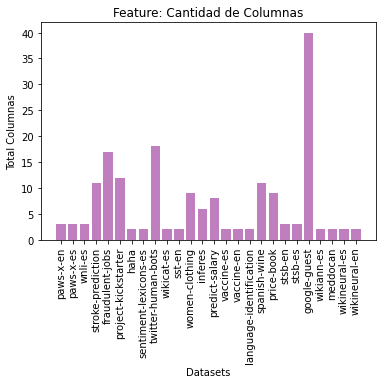
\includegraphics[width=\textwidth]{Graphics/results/columns.png}
        \caption{Número de Columnas}
        \label{fig:columns}
  \end{minipage}      
\hspace{0.01cm}
  \begin{minipage}[b]{0.31\textwidth}
    \centering
      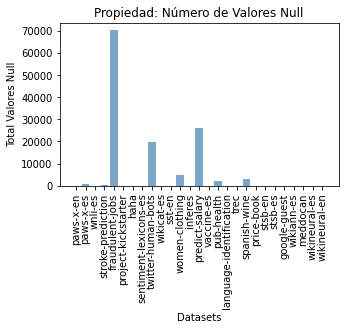
\includegraphics[width=\textwidth]{Graphics/results/null_values.png}
        \caption{Número de Nulls}
        \label{fig:null}
    \end{minipage} 
\end{figure}

\begin{figure}
  \centering
    \begin{minipage}[b]{0.31\textwidth}
        \centering
        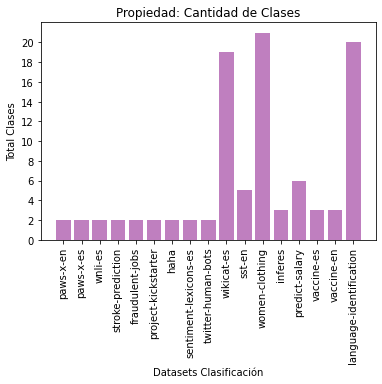
\includegraphics[width=\textwidth]{Graphics/results/class.png}
          \caption{Número de Clases}
          \label{fig:clases}
    \end{minipage}      
\hspace{0.03cm}
    \begin{minipage}[b]{0.31\textwidth}
        \centering
        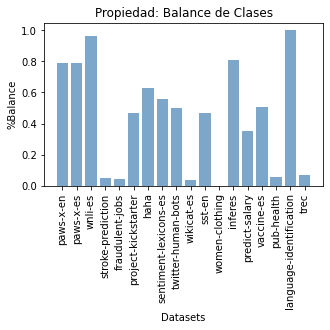
\includegraphics[width=\textwidth]{Graphics/results/balance.png}
          \caption{Índice de Balance}
          \label{fig:balance}
        \end{minipage} 
      \end{figure}

\begin{figure}
  \centering
    \begin{minipage}[b]{0.31\textwidth}
        \centering
        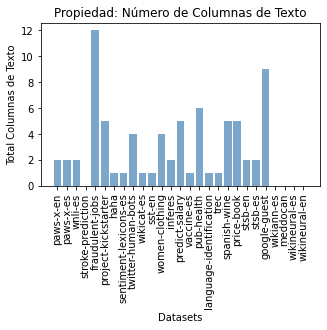
\includegraphics[width=\textwidth]{Graphics/results/columns_t.png}
          \caption{Tipo de Columna: Texto}
          \label{fig:columns-t}
    \end{minipage}      
\hspace{0.03cm}
    \begin{minipage}[b]{0.31\textwidth}
        \centering
        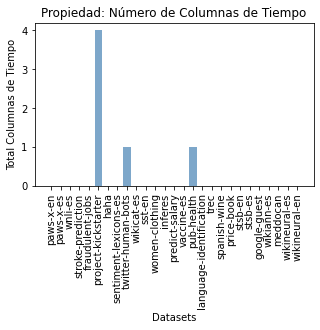
\includegraphics[width=\textwidth]{Graphics/results/columns_d.png}
          \caption{Tipo de Columna: Tiempo}
          \label{fig:columns-d}
        \end{minipage} 
\end{figure}

\begin{figure}
  \centering
    \begin{minipage}[b]{0.31\textwidth}
        \centering
        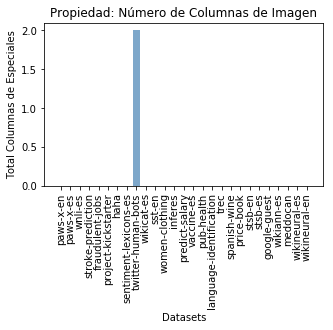
\includegraphics[width=\textwidth]{Graphics/results/columns_i.png}
          \caption{Tipo de Columna: Imagen}
          \label{fig:columns-i}
    \end{minipage}      
\hspace{0.03cm}
    \begin{minipage}[b]{0.31\textwidth}
        \centering
        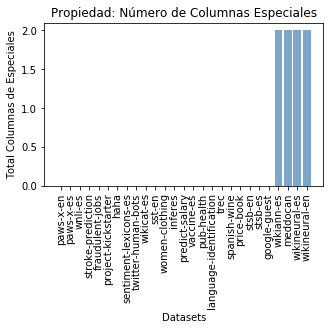
\includegraphics[width=\textwidth]{Graphics/results/columns_e.png}
          \caption{Tipo de Columna: Especial}
          \label{fig:columns-e}
        \end{minipage} 
\end{figure}

\begin{figure}
  \centering
    \begin{minipage}[b]{0.31\textwidth}
        \centering
        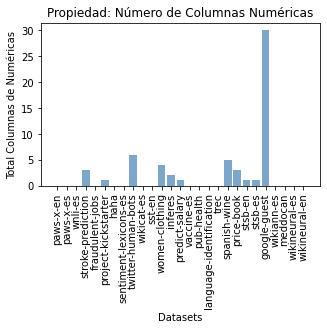
\includegraphics[width=\textwidth]{Graphics/results/columns_n.png}
          \caption{Tipo de Columna: Numérica}
          \label{fig:columns-n}
    \end{minipage}    
\hspace{0.01cm}
    \begin{minipage}[b]{0.31\textwidth}
      \centering
      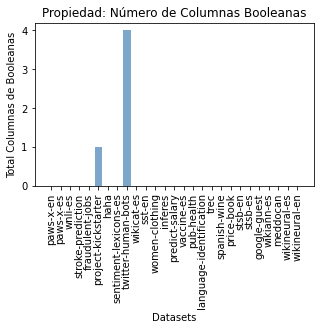
\includegraphics[width=\textwidth]{Graphics/results/columns_b.png}
        \caption{Tipo de Columna: Booleana}
        \label{fig:columns-b}
  \end{minipage}      
\hspace{0.01cm}
    \begin{minipage}[b]{0.31\textwidth}
        \centering
        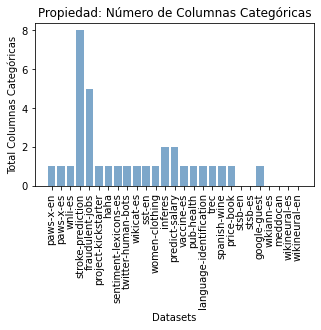
\includegraphics[width=\textwidth]{Graphics/results/columns_c.png}
          \caption{Tipo de Columna: Categórica}
          \label{fig:columns-c}
        \end{minipage} 
\end{figure}

\section{Evaluaciones Cualitativas}\label{section:qualitative}

En los últimos años, se han desarrollado una gran cantidad de sistemas Auto-ML, ya sea mediante la mejora iterativa de diseños antiguos o mediante 
el uso de enfoques novedosos. En el capítulo \ref{chapter:state-of-the-art} se explican algunas de las características de ciertos sistemas presentes en el 
estado del arte de Auto-ML. Entre estos sistemas se encuentran los Auto-DL: Auto-Keras [\cite{13}] y Auto-Pytorch [\cite{21}] y entre los Auto-ML clásicos: Auto-Weka, 
Auto-Sklearn, TPOT, AutoGluon, RECIPE y AutoGOAL.  
Esta sección se propone analizar cuáles de los sistemas anteriores según sus características pueden evaluarse en el benchmark.

\textit{HAutoML-Bench} agrupa conjuntos de gran complejidad, en su estructura y en sus datos, que requieren técnicas del dominio de aplicación para su utilización. 
Este benchmark va dirigido a sistemas Auto-ML que sean capaces de flexibilizar sus tipos de entrada 
y que contengan los algoritmos necesarios para evaluarse en los diferentes tipos de tareas que incluye. 

Los sistemas Auto-Weka, Auto-Sklearn, TPOT y RECIPE tienen como característica común que los datos de entrada deben contener solo características tabulares.
Los conjuntos del benchmark no evalúan esta cualidad de manera independiente de los demás tipos de datos. Además, incluyen una variedad de tipos de tareas como 
el reconocimiento de entidades y el procesamiento del lenguaje natural, que exigen técnicas del dominio al que pertenecen y los sistemas mencionados carecen de este tipo 
de técnicas. Estas propiedades afirman que estos 4 sistemas Auto-ML carecen de flexibilidad para evaluarse en todos los conjuntos de \textit{HAutoML-Bench}.

En el caso de los sistemas Auto-DL: Auto-Keras y AutoPytorch en sus respectivas evaluaciones incluyen pruebas en conjuntos de dominio imagen y tabular. 
A pesar de esto, el bechmark está desprovisto de conjuntos que solamente respondan a esos dominios. Auto-Keras al tener componentes para tratar con dominio texto y problemas 
multimodales, es un software en potencia para ser evaluado en el benchmark. Sin embargo, en las evaluaciones que muestran sus capacidades solo se prueba 
en conjuntos juguetes que sufren de falta de semántica al estar transformados. AutoPytorch no tiene de técnicas de procesamiento para el dominio texto y 
tampoco permite la multimodalidad.
En conclusión, no existe evidencia de que estos sistemas pueda evaluarse en conjuntos con tipos de datos no estructurados como los que incluye 
\textit{HAutoML-Bench} . 

El sistema AutoGOAL al implementar tipos semánticos permite tener variedad en la estructura de su entrada y salida, por lo que pueden evaluarse tipos estructurados y no
estructurados. Además, posee técnicas para resolver tareas relacionadas con el dominio texto incluidas las tareas de extracción de entidades. Este ,en su 
documentación, se evalúa en dos de los conjuntos de datos de \textit{HAutoML-Bench} meddocan y haha, lo que permite afirmar que es posible evaluarlo en las tareas 
relacionadas con el dominio texto que pertenecen al benchmark. Sin embargo, en conjuntos de datos multimodales carecen de un tipo definido que permita modelar estas entradas.    

AutoGluon posee técnicas para procesar entradas de texto, imágenes, tabulares y series temporales y estas entradas pueden encontrarse estructuradas o no. Además, con su 
modelo multimodal es capaz de resolver problemas en donde existe una mezcla de los tipos de datos de imágenes, texto y tabulares y cada uno puede encontrarse a gran escala.
Se puede decir que por sus propiedades, AutoGluon está preparado para enfrentarse a los conjuntos multimodales y de texto de \textit{HAutoML-Bench}, excepto las 
tareas de reconocimiento de entidades. AutoGluon tiene técnicas para tratar las tareas de reconocimiento de entidades; sin embargo, la entrada para este tipo de 
problemas presentan una estructura diferente a las que poseen los conjuntos de \textit{HAutoML-Bench}


En la figura \ref{fig:eval-cuali} se muestra un resumen de los tipos y dominios de las tareas que potencialmente cada sistema puede resolver. 
\begin{table}[H]
  \centering
  \resizebox{14cm}{!} {
  \begin{tabular}{|c|c|c|c|c|c|}
  \hline
  Auto-ML & \multicolumn{3}{c|}{Texto} & \multicolumn{2}{c|}{Multimodales}\\ 
  \cline{2-6}
                        & tarea clasificación   & tarea regresión   & tarea entidades& tarea clasificación   & tarea regresión   \\ \hline
  Auto-Weka             &          &          &          &          &          \\
  Auto-Sklearn          &          &          &          &          &          \\
  TPOT                  &          &          &          &          &          \\ 
  RECIPE                &          &          &          &          &          \\
  AutoPytorch           &          &          &          &          &          \\
  Auto-Keras            &          &          &          &          &          \\
  AutoGOAL              &\checkmark&\checkmark&\checkmark&          &          \\
  AutoGluon             &\checkmark&\checkmark&          &\checkmark&\checkmark\\ \hline
  Total &  10      &  2       &  4       &   8      &  3       \\ \hline
  \end{tabular}
  \caption{Evaluación Cualitativa de los sistemas sobre los conjuntos de datos del benchmark}
  \label{fig:eval-cuali}
  }
\end{table}

\section{Evaluaciones Cuantitativas}\label{section:quantitative}

Las evidencias presentadas en el apartado (\ref{section:qualitative}) permiten concluir que AutoGOAL y AutoGluon atendiendo a sus características pueden 
evaluarse en 16 y 23 conjuntos de \textit{HAutoML-Bench} respectivamente.
Para la evaluación cuantitativa, el sistema seleccionado es AutoGluon. Este posee potencialmente la mayor cantidad de tareas que sus características afirman 
puede resolver. 
La selección incluye solo uno de los sistemas debido a limitantes de tiempo y software. 
En las próximas subsecciones se explica todo el marco experimental cuantitativo que pone a prueba el rendimiento de AutoGluon (\ref{subsection:seetings}). Se muestran 
los resultados del rendimiento del sistema (\ref{subsection:results}) y se explican los errores que surgieron en las evaluaciones (\ref{subsection:errors})

\subsection{Descripción y Configuración de las Evaluaciones}\label{subsection:seetings}

La experimentación cuantitativa propone realizar tres rondas de evaluaciones de AutoGluon sobre todos los conjuntos de datos.

El hadware de evaluación seleccionado es la plataforma Colab[\cite{colab}]. Esta cuenta con un entorno de ejecución en la nube que provee recursos para ejecutar programas 
escritos en el lenguaje Python. Los recursos presentes en la evaluación son: CPU de 12 GB de RAM máximo, 120 GB de almacenamiento de disco duro y 188 unidades de GPU.
AutoGluon se utiliza en su versión estable v0.5.2. Esta herramienta tiene muchos parámetros configurables en cada uno de sus modelos, tabular, multimodal, imagen y texto. 
Estos presentan su configuración predeterminada, exceptuando los que se describen a continuación:

\begin{itemize}
    \item Restricciones de software: La herramienta se instala con GPU, en vista a verificar su rapidez y rendimiento durante las pruebas. No existen limitaciones de RAM salvo
    las impuestas por el entorno de ejecución.
    \item Métrica de optimización: Se utilizan para clasificación binaria: \textit{F1}, clasificación multiclase: \textit{accuracy} y para regresión \textit{RMSE}. Todas se 
    encuentran dentro de las métricas medidas en la evaluación. Se emplean estas y no las ideales recomendadas porque AutoGluon es restrictivo con las métricas que 
    pueden utilizarse en cada modelo. La \textit{balanced-accuracy} está fuera de las permitidas.
    \item Restricciones de tiempo: selección de dos instantes de tiempo para la realización de las evaluaciones 5 y 15 minutos.
    \item Tamaño del conjunto de validación: utilizar un tamaño 0.2 del total de instancias que equivale a un 20\%. 
    \item Parámetros obligatorios: la etiqueta de la columna salida.  
  \end{itemize}
  
  La primera ronda tiene como objetivo medir el rendimiento de AutoGluon con todos sus parámetros de entrada en sus valores por defecto. En esta solo se especifican los 
  relacionados con la métrica de optimización y el tiempo de 5 minutos. 
  
  La segunda ronda pretende evaluar el sistema en las mismas condiciones de la primera ronda, excepto por el tiempo que superar el anterior; 15 minutos.
  Estas primeras etapas de ejecuciones tienen como fin evaluar al sistema realizando su propia inferencia de tipos, se pretende que la herramienta obtenga la mínima
  ayuda externa. La segunda además pretende verificar si el rendimiento de la herramienta es sensible a los cambios de tiempo, posibilitando alguna 
  mejora en la mayoría de los conjuntos.
  
  En la última ronda se introducen como entrada los tipos semánticos de cada columna de los conjuntos. La meta es validar la consistencia de los resultados de 
  AutoGluon en comparación con los obtenidos con inferencia de tipos durante el mismo tiempo de entrenamiento: 5 minutos. 

\subsection{Resultados}\label{subsection:results}

Los valores obtenidos durante cada una de las etapas de evaluación se muestran en esta sección. Los resultados se encuentran separados en los diferentes tipos de tareas
en las figuras \ref{fig:class-binary}, \ref{fig:class-multi} y \ref{fig:regression} que corresponden a clasificación binaria, multiclase y regresión.  

Las métricas de evaluación que se muestran para cada tarea es la utilizada para la optimización del sistema y además se muestra la métrica ideal propuesta en la 
sección(\ref{subsection:metrics}).
En el caso de la regresión, los valores de la variable de salida no se encuentran en el mismo rango, ni los resultados obtenidos en la métrica \textit{RMSE} 
durante la evaluación del benchmark. Producto a esto, los valores del error de los conjuntos impiden su comparación. Para resolver este inconveniente,
como evaluación independiente\footnote{Los resultados originales junto a las otras métricas que se excluyeron en esta descripción se encuentran en el repositorio del 
benchmark.} se estandarizan los valores de las variables de salida y las predicciones de cada conjunto de regresión, luego se calcula la métrica 
\textit{RMSE}.

En las figuras (\ref{fig:class-binary}, \ref{fig:class-multi}, \ref{fig:regression}) tambíen se muestra el promedio de los resultados de cada métrica en cada tarea. 
Este promedio permite analizar de manera general los cambios que sufren los valores de rendimiento del sistema en las 3 etapas de evaluaciones.

En esta sección se ofrece una descripción de los resultados de todas las etapas de la evaluación, en cada uno de los tipos de tareas por 
separado (\ref{results:task}). 
Luego se compara el rendimiento del sistema en las distintas etapas (\ref{results:comparation}). Las comparaciones se efectúan entre las etapas que 
mantienen sus parámetros por defecto y existe un aumento del tiempo (etapa 1 y 2), y cuando se mantiene el mismo tiempo y lo que varía es la introducción de los 
tipos de las columnas de entrada (etapa 1 y 3).


\begin{flushleft} 
  {\large { \textbf{Resultados de AutoGluon por Tipo de Tarea}}}\label{results:task}
\end{flushleft}

Los resultados en las distintas tareas se manifiestan similares en cada una de las etapas. Esta similitud es teniendo en cuenta los mejores y peores conjuntos en 
rendimiento.

En la clasificación, atendiendo a los valores de la métrica \textit{balanced-accuracy}, que es común en ambos tipos de clasificaciones, el mayor promedio de desempeño durante todas las rondas de 
evaluación lo posee la clasificación binaria.
En esta tarea, el conjunto en el que AutoGluon tiene mejor rendimiento durante todos las evaluaciones es \textit{paw-x-en}. Los peores resultados varían en dependencia de la etapa y la 
métrica. El que más resalta es \textit{stroke-prediction} que posee un valor de \textit{F1} igual a cero durante todas las etapas. Las evaluaciones del conjunto 
\textit{fradulent-job} tienen un comportamiento similar, excepto en la etapa 2 en donde aumenta el valor de su rendimiento. En la métrica \textit{balanced-accuracy} 
los conjuntos> \textit{project-kickstarter} y \textit{wnli-es} se unen a aquellos en donde el rendimiento es malo.

En la clasificación multiclase, al igual que en la clasificación binaria, existe un conjunto en donde la herramienta tiene buenos resultados durante todas las rondas de 
ejecuciones, este es \textit{language-identification}. En la tercera ronda de evaluaciones el mejor rendimiento es compartido con \textit{trec}. El peor desempeño 
durante todo el proceso es en el conjunto \textit{predict-salary}.

En la tarea regresión los mejores resultados se obtienen en el conjunto \textit{stsb-en}, mientras que el error es mayor en \textit{price-book} en todas las rondas 
de ejecuciones.


\begin{flushleft} 
  {\large { \textbf{Comparación de los Resultados de las Etapas de Evaluación de AutoGluon}}}\label{results:comparation}
\end{flushleft}

Los resultados del sistema, con sus parámetros de entrada por defecto, muestran un promedio de desempeño superior en 15 minutos que en 5 minutos. 
En todos los conjuntos de clasificación binaria, AutoGluon aumenta su rendimiento con el incremento del tiempo. 
Las mayores variaciones en este tipo de tareas son en los conjuntos \textit{fradulent-job} y \textit{project-kickstarter}, mientras que \textit{stroke-prediction}, 
es el único en donde no se observa una variación en sus resultados.

En la clasificación multiclase existe una disminución del rendimiento del sistema  a medida que aumenta el tiempo en los conjuntos: \textit{predict-salary} y 
\textit{vaccine-es}. En todos los conjuntos restantes de esta categoría, sus valores de eficiencia muestran un aumento, el mayor de todos es en el 
conjunto \textit{wikicat-es}.
En las dos tareas de clasificación, el cambio en los valores de eficiencia de un tiempo a otro es más significativo en la clasificación binaria.
En estas etapas, las tareas de regresión  mejoran sus resultados en todos sus conjuntos, excepto \textit{price-book}.

AutoGluon con la introducción de los tipos de datos de las columnas de los conjuntos en la etapa 3, no muestra una gran variación en sus resultados.
Este en la mayoría de los ejemplos tiende a mantener o disminuir su eficiencia al tener como entrada los tipos de las columnas. Los conjuntos en los que muestra un 
notable incremento en su rendimiento son: \textit{project-kickstarter} en clasificación binaria, en multiclase \textit{women-clothing} y regresión 
\textit{google-guest}. Estos grandes incrementos provocan que el promedio de rendimiento de la tercera etapa sea mayor al de la primera. Si bien el promedio es mayor, 
esto no significa que para los conjuntos sea favorable el introducir como entrada el tipo de las columnas. 
AutoGluon en la tarea regresión muestra su mayor disminución de eficiencia de una etapa a la otra en el conjunto \textit{spanish-wine}.

\begin{table}
  \centering
  \resizebox{15cm}{!} {
  \begin{tabular}{|c|cccccc|}
  \hline
  Conjuntos & \multicolumn{4}{P{8cm}|}{Tiempo: 5 min}  & \multicolumn{2}{P{4cm}|}{Tiempo: 15 min}\\  
    \cline{2-7}
  & \multicolumn{2}{P{4cm}|}{Entrada Valores} & \multicolumn{2}{P{4cm}|}{Entrada: Tipos} & \multicolumn{2}{P{4cm}|}{Entrada Valores}\\ 
  & \multicolumn{2}{P{4cm}|}{por Defecto} & \multicolumn{2}{P{4cm}|}{Semánticos} & \multicolumn{2}{P{4cm}|}{por Defecto}\\    
  \cline{2-7}
           & F1 & bala-acc & F1  & bal-acc & F1 & bal-acc  \\ \hline
  paws-x-en             & 0.931 & 0.940 & 0.917 & 0.928 & 0.947 & 0.953 \\
  paws-x-es             & 0.840 & 0.856 & 0.837 & 0.852 & 0.875 & 0.888 \\
  wnli-es               & 0.61  & 0.5   & 0.613 & 0.5   & 0.613 & 0.5   \\ 
  stroke-prediction     & 0.0   & 0.5   & 0.0   & 0.5   & 0.0   & 0.5 \\
  fraudulent-jobs       & 0.0   & 0.5   & 0.0   & 0.5   & 0.732 & 0.818 \\
  project-kickstarter   & 0.074 & 0.498 & 0.225 & 0.499 & 0.153 & 0.502 \\
  haha                  & 0.764 & 0.807 & 0.761 & 0.803 & 0.774 & 0.814 \\
  sentiment-lexicons-es & 0.747 & 0.770 & 0.747 & 0.770 & 0.775 & 0.794 \\ 
  twitter-human-bots    & 0.680 & 0.770 & 0.676 & 0.759 & 0.721 & 0.791 \\ \hline
  \textbf{Promedio}     & 0.516 & 0.682 & 0.530 & 0.679 & 0.621 & 0.728 \\ \hline


  \end{tabular}
  \caption{Resultados en tareas de Clasificación Binaria:
  \\Se muestran los valores de las métricas F1 y balanced-accuracy en cada una de las rondas de evaluación}
  \label{fig:class-binary}
  }
\end{table}

\begin{table}
  \centering
  \resizebox{15cm}{!} {
    \begin{tabular}{|c|cccccc|}
   \hline
   Conjuntos & \multicolumn{4}{P{8cm}|}{Tiempo: 5 min}  & \multicolumn{2}{P{4cm}|}{Tiempo: 15 min}\\  
    \cline{2-7}
          & \multicolumn{2}{P{4cm}|}{Entrada Valores} & \multicolumn{2}{P{4cm}|}{Entrada: Tipos} & \multicolumn{2}{P{4cm}|}{Entrada Valores}\\ 
          & \multicolumn{2}{P{4cm}|}{por Defecto} & \multicolumn{2}{P{4cm}|}{Semánticos} & \multicolumn{2}{P{4cm}|}{por Defecto}\\ 
    \cline{2-7}
                 & acc & bala-acc & acc  & bal-acc & acc & bal-acc  \\ \hline
  wikicat-es              & 0.385 & 0.268 & 0.385 & 0.268 & 0.603 & 0.518 \\
  sst-en                  & 0.580 & 0.549 & 0.580 & 0.549 & 0.577 & 0.545 \\
  women-clothing          & 0.671 & 0.449 & 0.677 & 0.456 & 0.760 & 0.642 \\ 
  inferes                 & 0.691 & 0.680 & 0.651 & 0.647 & 0.767 & 0.759 \\
  predict-salary          & 0.199 & 0.178 & 0.190 & 0.173 & 0.191 & 0.172 \\
  language-identification & 0.966 & 0.966 & 0.966 & 0.966 & 0.976 & 0.976 \\
  vaccine-es              & 0.780 & 0.756 & 0.779 & 0.743 & 0.779 & 0.766 \\
  pub-health              & 0.609 & 0.370 & 0.609 & 0.370 & 0.759 & 0.576 \\ 
  trec                    & 0.962 & 0.912 & 0.966 & 0.933 & 0.970 & 0.972 \\ \hline
  \textbf{Promedio}       & 0.649 & 0.569 & 0.723 & 0.567 & 0.684 & 0.658 \\ \hline


    \end{tabular}
  \caption{Resultados en tareas de Clasificación Multiclase:
  \\Se muestran los valores de las métricas accuracy y balanced-accuracy en cada una de las rondas de evaluación}
  \label{fig:class-multi}
  }
\end{table}

\begin{table}[H]
  \centering
  \resizebox{15cm}{!} {
  \begin{tabular}{|c|ccc|}
  \hline
  Conjuntos & \multicolumn{2}{P{8cm}|}{Tiempo: 5 min}  & \multicolumn{1}{P{4cm}|}{Tiempo: 15 min} \\ 
  \cline{2-4}
  & \multicolumn{1}{P{4cm}|}{Entrada Valores} & \multicolumn{1}{P{4cm}|}{Entrada Tipos} & \multicolumn{1}{P{4cm}|}{Entrada Valores}\\ 
  & \multicolumn{1}{P{4cm}|}{ por Defecto} & \multicolumn{1}{P{4cm}|}{Semánticos} & \multicolumn{1}{P{4cm}|}{por Defecto}\\ 
  \cline{2-4}
               & RMSE  & RMSE  & RMSE  \\ \hline
  spanish-wine & 0.8274  & 36.62  & 0.5581 \\
  stsb-en      & 0.4548  & 0.472  & 0.4349 \\
  stsb-es      & 0.6265  & 0.6265 & 0.6231   \\ 
  price-book   & 32.537  & 40.675 & 40.864  \\
  google-guest & 1.7156  & 1.5171 & 1.5355  \\ \hline
  \textbf{Promedio} & 0.1741 & 0.1652 & 0.1556 \\ \hline

\end{tabular}
  \caption{Resultados en tareas de Regresión:
  \\Se muestran los valores de la métrica RMSE en cada una de las rondas de evaluación}
  \label{fig:regression}
  }
\end{table}


\subsection{Fallas de Evaluación}\label{subsection:errors}
AutoGluon,el sistema Auto-ML evaluado, presenta fallas durante las ejecuciones de algunos conjuntos. Estos para poder evaluarse tienen que ser sometidos a 
transformaciones.
El conjunto \textit{women-clothing} contiene una clase que solo posee una instancia. También, posee valores faltantes en su columna salida. En ambos casos AutoGluon no 
puede resolver problemas de este tipo. Para que el sistema pueda ejecutarse, las instancias con problemas son removidas.

El conjunto \textit{google-guest} tiene en su etiqueta final un número de valores distintos, bastante pequeño. En su definición original este modela una tarea de regresión y en 
los valores de la etiqueta final pueden estar en el rango [0,1]. El sistema infiere incorrectamente el tipo de tarea, lo que produce errores en la ejecución, para 
dar una solución se introduce el tipo de tarea, solamente para este conjunto.

Estas ejecuciones fallidas ocurren durante la primera ronda de pruebas. Las soluciones a estos problemas deben ser reutilizadas en las restantes rondas. 
En la última, ocurren errores al introducir los tipos semánticos de cada una de las columnas. Las primeras limitaciones se dan al no poder introducir como 
parámetro de entrada el tipo \textit{datetime}, que hace referencia a los tipos de tiempo y fecha. Además, en el procesamiento del tipo \textit{path\_image} de AutoGluon. 
Este solo permite imágenes ubicadas en un directorio, carece de la funcionalidad de descargar imágenes de una url. Estos tipos fueron apartados de la entrada.

El conjunto \textit{spanish-wine} en sus entradas etiquetadas como numéricas y que presentan datos faltantes AutoGluon detiene la ejecución. Al ser pocas instancias 
se remueven.
En el caso de \textit{price-book} contiene columnas que su tipo semántico es numeral y su tipo concreto es cadena de texto. AutoGluon carece de técnicas para 
enfrentarse a este tipo de situaciones. En este ejemplo se transformaron las columnas a números y se le pasaron al sistema de esa forma.
En todas las rondas de evaluaciones existieron errores de falta de RAM al ejecutar algunos conjuntos.

\section{Discusión}\label{subsection:discussions}

Las evaluaciones cuantitativas y cualitativas realizadas en las secciones (\ref{section:quantitative}) y (\ref{section:qualitative}) denotan la complejidad que poseen 
los conjuntos de \textit{HAutoML-Bench}.
El análisis que se realiza sobre sus propiedades ya habían anticipado su dificultad, producto a los tipos de datos no estructurados que poseen y a sus 
metacaracterísticas.

Las evaluaciones cualitativas evidencian que en su mayoría los sistemas Auto-ML son incapaces de evaluar su eficiencia en los conjuntos de \textit{HAutoML-Bench}. 
En los casos de la herramienta AutoDL, que ya poseen técnicas para procesar tareas de un dominio específico, deben agregar técnicas para lidiar con datos no estructurados. 
En los ejemplos de sistemas Auto-ML que solo se ejecutan en datos tabulares, deben superar esta limitante con el fin de lograr la heterogeneidad. 
El sistema AutoGOAL debe añadir más tipos semánticos para poder evaluarse en conjuntos multimodales. AutoGluon debe ampliar las formas en que recibe el tipo de entrada 
de las tareas de reconocimiento de entidades.

AutoGluon es el sistema con características más maduras que permiten la evaluación en 23 conjuntos de datos de \textit{HAutoML-Bench}.
Los resultados de su evaluación cuantitativa presenta algunas de las deficiencias que este sistema aún posee. Además, resalta sus fortalezas, ya que obtuvo buenos resultados 
en algunos casos.
%Los valores de rendimiento que obtiene el sistema, buenos o malos, se agrupan, atendiendo a las características que presentan los datos en cada conjunto.

Los buenos resultados del sistema suelen ser en conjuntos con un índice de balance elevado en sus clases. Ejemplo son \textit{paws-x-en} y 
\textit{language-identification} que son los más balaceados de \textit{HAutoML-Bench}. El idioma inglés parece ser otra ventaja para el buen rendimiento, ya que
existen conjuntos creados para el idioma español e inglés y AutoGluon obtiene una mayor eficiencia en los de idioma inglés.

El desbalance de clase y los conjuntos multimodales parecen ser la mayor fuente de ineficiencia. Ejemplos son los conjuntos \textit{stroke-prediction} y 
\textit{fraudulent-job}, que mantienen un rendimiento bastante bajo e invariante, prediciendo correctamente solo la clase negativa. El conjunto \textit{fraudulent-job} 
en un intervalo mayor de tiempo que el inicial logra aumentar sus resultados, a pesar de ser un conjunto con muchos valores faltantes. AutoGluon parece 
enfrentar bien estos faltantes cuando la característica no se especifica como numérica. Otra desventaja es los 
pocos datos de entrenamiento. Los conjuntos \textit{Wnli-es} y \textit{stroke-prediction} son muestra de esta deficiencia. \textit{Wnli-es}, al 
contrario de los anteriores conjuntos mencionados, tiende a predecir con mayor frecuencia la clase positiva.

El conjunto \textit{price-book} es ejemplo del aumento del error en tareas de regresion producto al rango elevado de los valores de su variable de salida y a sus 
propiedades multimodales. En las tareas de clasificación multiclase, se repiten los bajos rendimientos
en tareas multimodales, con valores faltantes y desbalance de clase. Ejemplo el conjunto \textit{predict-salary} que obtiene los resultados más bajos de esta tarea. 
Cada uno de los valores de desempeño demuestran la superioridad del rendimiento de AutoGluon en tareas de texto puro sobre las multimodales. 

Con respecto a los objetivos de cada etapa de evaluación. En aquellas donde se comparan los resultados con diferente tiempo, AutoGluon demuestra un aumento en 
su rendimiento. Se estima que el tiempo máximo de entrenamiento es suficiente para completar las tareas, considerando que todos los conjuntos se evalúan con GPU y que 
logran alcanzar como mínimo la etapa 2 de entrenamiento. En este tiempo, los resultados por tarea presentan un promedio menor al 75 por ciento, este valor comparado 
con las épocas de entrenamiento, es ineficiente. 

En las comparaciones en donde se quiere verificar la fortaleza de la inferencia de tipos, AutoGluon muestra que no existen variaciones drásticas entre las etapas 
comparadas. Existen conjuntos en donde el sistema disminuye su rendimiento cuando se introducen los tipos de entrada. Esto afirma que los tipos que se infieren, 
en muchos casos, no coincide con el correcto, a pesar de ello, AutoGluon se las ingenia para obtener un resultado medio.


